\documentclass[../main.tex]{subfiles}

\begin{document}
	
		
	\section*{Abstract}
	McMurty und Sanders entwickelten in 1985 das erste kommerzielle Aquaponiksystem mit Tilapia-Buntbarschen mit der sie die Aufzucht von Tomaten aufbereiteten. Bei Aquaponik handelt es sich um den Kreislauf zwischen Aquakultur und Hydroponik. Aquakultur steht für die Zucht von Wassertieren in einem Becken und Hydroponiks steht für die pflanzliche Kultivierung. Heutzutage sind kleine und grosse Aquaponiksysteme überall auf der Welt anzutreffen und finden sowohl in Industrie- und Entwicklungsländern ihre Verwendung. Um ein gesundes Leben der Fische und eine gute Ernte zu garantieren, müssen die Tiere, die Pflanzen und vor allem das Wasser gut überwacht werden. Die Überwachung wird mit vielen verschiedenen Sensoren automatisiert, welche auch bei der Forschung bei der ZHAW Life Sciences und Facility Management der Fall ist. Nun handelt es sich hierbei um Labore und Testsysteme die öfters mal neu oder umgebaut werden, welche eine Neukonfiguration der Sensoren benötigt. Bei dieser trägen und fehlerhaften Arbeit sollen wir ein Tool entwickeln, welches das Eintragen und Auslesen von den Sensoren vereinfacht.\\
	
	\begin{figure}[H]
		\centering
		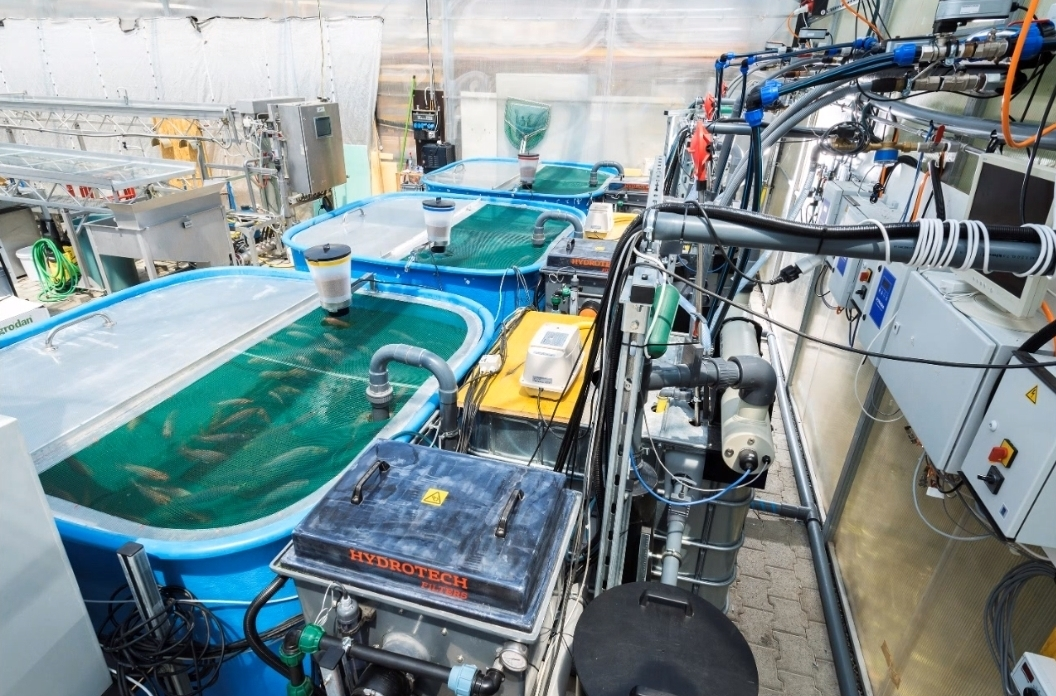
\includegraphics[scale=0.5]{Aquaponics_Tank}
		\caption{Tank in Wädischwil}
		\label{fig:Aquaponics_Tank}
	\end{figure}
	\par \noindent
	
\end{document}